\documentclass{beamer}

\usetheme{Madrid}
\usecolortheme{beaver}

\usepackage[utf8]{inputenc}
\usepackage[brazil]{babel}
\usepackage{amsmath, amssymb}
\usepackage{booktabs}
\usepackage{array}
\usepackage{graphicx}
\usepackage{tcolorbox}
\usepackage{hyperref}
\usepackage{tikz}
\usetikzlibrary{arrows.meta, positioning}

\tcbuselibrary{skins, breakable}

\AtBeginSection[]
{
  \begin{frame}
    \frametitle{Índice}
    \tableofcontents[currentsection]
  \end{frame}
}

\newcommand{\R}{\mathrm{R}}
\newcommand{\A}{\mathrm{A}}
\newcommand{\MTTF}{\mathrm{MTTF}}
\newcommand{\MTBF}{\mathrm{MTBF}}
\newcommand{\MTTR}{\mathrm{MTTR}}

\title[Confiabilidade e Disponibilidade]{Dependabilidade: Confiabilidade e Disponibilidade}
\subtitle{MTBF, MTTR, MTTF, \texorpdfstring{$\R(t)$}{R(t)} e disponibilidade}
\author{Prof. Iaçanã Ianiski Weber}
\institute{PUCRS}
\date[]{}

\begin{document}

\begin{frame}[plain]
\noindent
\begin{minipage}[t]{0.15\textwidth}
    
\includegraphics[width=\linewidth]{../img/brasao_pucrs.png}
\end{minipage}%
\begin{minipage}[t]{0.75\textwidth}
    \begin{center}
        \raisebox{5ex}{\LARGE\bfseries\textcolor{blue}{\textbf{Dependabilidade:}}}\\
        \raisebox{2ex}{\LARGE\bfseries\textcolor{blue}{Confiabilidade e Disponibilidade}}\\
    \end{center}
\end{minipage}

\vspace{1.4cm}

\begin{center}
    \Large \textbf{Prof. Dr. Iaçanã Ianiski Weber} \\
    \vspace{0.2cm}
    \normalsize \textit{Confiabilidade e Segurança de Software} \\
    \vspace{0.2cm}
    \large 98G08-4
\end{center}
\end{frame}

\begin{frame}{Objetivos de aprendizagem}
Ao final desta aula, você deve conseguir:
\begin{enumerate}
  \item Definir dependabilidade e explicar por que \textbf{confiabilidade} não é igual a \textbf{disponibilidade}.
  \item Diferenciar e calcular \(\MTBF\), \(\MTTR\) e \(\MTTF\) (quando aplicável).
  \item Calcular disponibilidade \(\A\) e estimar indisponibilidade anual (SLA).
  \item Resolver problemas simples com \(\R(t)\) e \(\A\), interpretando o resultado.
\end{enumerate}
\end{frame}

\begin{frame}{Plano da aula}
\small
\centering
\begin{tabular}{p{0.32\textwidth} p{0.62\textwidth}}
\toprule
\textbf{Bloco} & \textbf{Conteúdo} \\
\midrule
Fundamentos & Dependabilidade, motivação e mapa de atributos \\
Confiabilidade & Fundamentos probabilísticos e interpretação de \(F(t)\), \(R(t)\), \(f(t)\) \\
Disponibilidade & \(\MTTR\), \(\A \approx \frac{\MTBF}{\MTBF+\MTTR}\), SLA e downtime \\
Verificação & Perguntas de interpretação técnica \\
Exercícios & Lista com resolução guiada \\
Fechamento & Síntese e gancho para a próxima aula \\
\bottomrule
\end{tabular}
\end{frame}

\section{Fundamentos}

\begin{frame}{Por que isso importa?}
\begin{itemize}
  \item Sistemas reais falham: software, infraestrutura, rede e operação humana.
  \item A pergunta de engenharia não é só \textit{``vai falhar?''}, mas:
  \begin{itemize}
    \item \textbf{Com que frequência falha?} (confiabilidade)
    \item \textbf{Quanto tempo fica fora?} (disponibilidade)
  \end{itemize}
\end{itemize}

\begin{block}{Exemplo curto}
Sistema X cai raramente, mas demora para voltar.\\
Sistema Y cai mais, mas volta quase instantaneamente.\\
\textbf{Qual experiência de usuário pode ser melhor?} Depende de \(\MTBF\) e \(\MTTR\).
\end{block}
\end{frame}

\begin{frame}{Dependabilidade: definição operacional e mapa}
\begin{block}{Dependabilidade}
Propriedade de um sistema entregar serviço correto e confiável ao longo do tempo, apesar de falhas.
\end{block}

\begin{center}
\resizebox{0.90\linewidth}{!}{
\begin{tikzpicture}[
  node distance=2.0cm,
  core/.style={draw, rounded corners=2mm, thick, fill=blue!8, minimum width=3.4cm, minimum height=1.2cm, align=center},
  attr/.style={draw, rounded corners=1.5mm, thick, fill=gray!10, minimum width=3.0cm, minimum height=0.95cm, align=center},
  arrow/.style={-Latex, thick, color=black!70}
]
  \node[core] (sys) {Sistema\\(serviço correto)};
  \node[attr, above left=1.0cm and 2.2cm of sys] (conf) {\textbf{Confiabilidade}};
  \node[attr, above right=1.0cm and 2.2cm of sys] (disp) {\textbf{Disponibilidade}};
  \node[attr, below left=1.0cm and 2.2cm of sys] (safe) {Safety};
  \node[attr, below right=1.0cm and 2.2cm of sys] (sec) {Security};
  \node[attr, below=2.2cm of sys] (res) {Resiliência};

  \draw[arrow] (sys) -- (conf);
  \draw[arrow] (sys) -- (disp);
  \draw[arrow] (sys) -- (safe);
  \draw[arrow] (sys) -- (sec);
  \draw[arrow] (sys) -- (res);
\end{tikzpicture}
}
\end{center}
\end{frame}

\section{Confiabilidade}

\begin{frame}{Confiabilidade: visão geral}
\begin{itemize}
  \item Nesta parte, pense em 3 perguntas:
  \begin{enumerate}
    \item Quando a falha acontece? (tempo até falha)
    \item Qual a chance de já ter falhado até \(t\)?
    \item Qual a chance de ainda estar funcionando em \(t\)?
  \end{enumerate}
  \item O foco é \textbf{intuição + conta prática}, sem aprofundar em estatística pesada.
\end{itemize}
\end{frame}

\begin{frame}{Passo 1: TTF como variável aleatória}
\begin{block}{TTF (Time To Failure)}
TTF é o tempo até a primeira falha.
\end{block}
\begin{itemize}
  \item Cada equipamento falha em um tempo diferente.
  \item Por isso, \(T\) é tratado como variável aleatória.
  \item Ex.: um item falha em 80h, outro em 130h, outro em 210h.
\end{itemize}
\begin{block}{Leitura intuitiva}
Não buscamos o tempo exato de um item, e sim o comportamento probabilístico do conjunto.
\end{block}
\centering
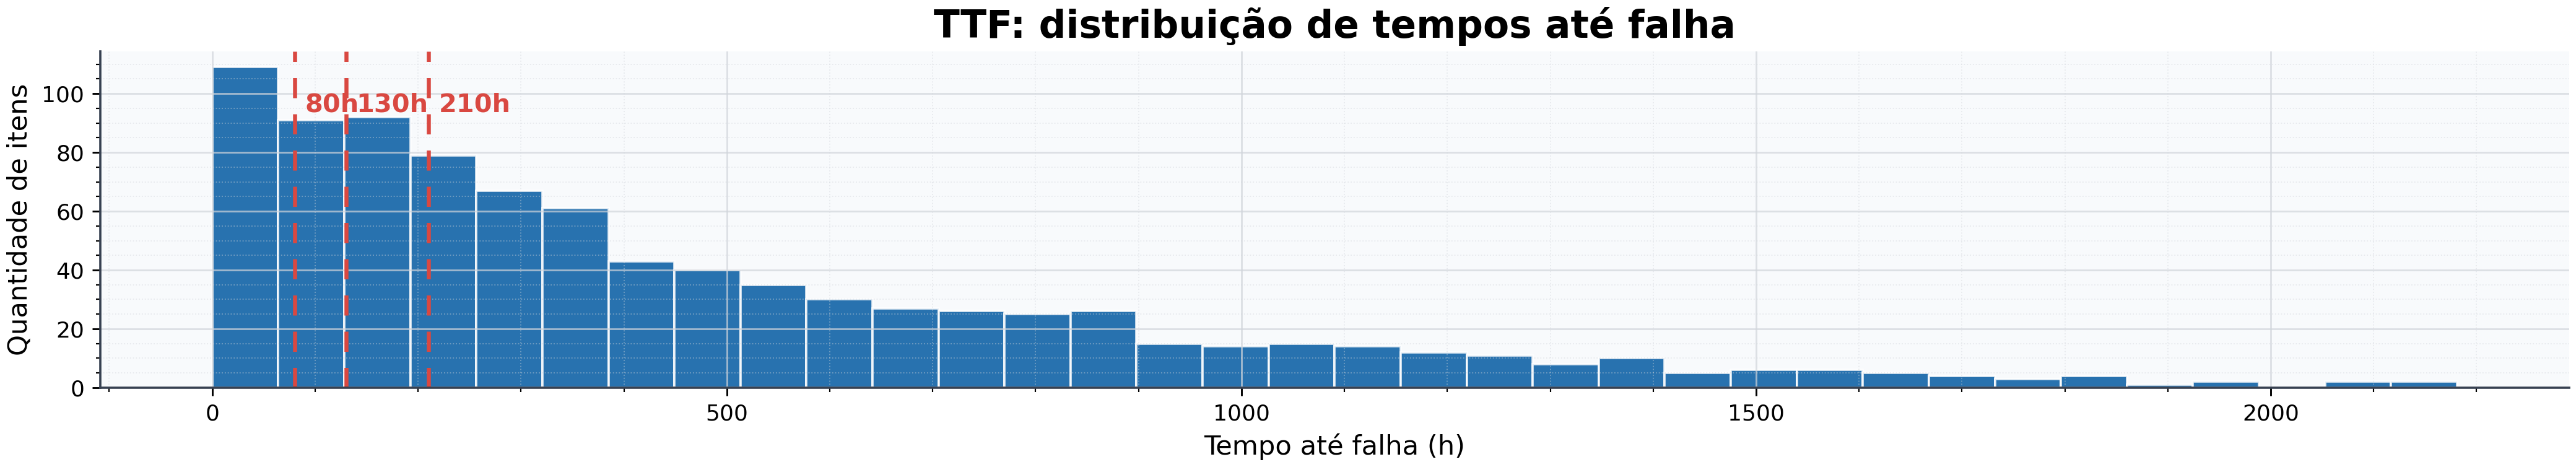
\includegraphics[width=\linewidth,height=0.35\textheight,keepaspectratio]{../img/unit2_ttf_samples_wide.png}
\end{frame}

\begin{frame}{Passo 2: função acumulada \texorpdfstring{$F(t)$}{F(t)}}
\[
F(t)=P(T\le t)
\]
\begin{itemize}
  \item Leitura: probabilidade de o sistema \textbf{já ter falhado} até o instante \(t\).
  \item Exemplo: \(F(100)=0.20\) significa 20\% de chance de falhar até 100h.
\end{itemize}

\begin{block}{Regra rápida}
Quanto maior o tempo \(t\), maior (ou igual) tende a ser \(F(t)\), pois você acumula mais chance de falha.
\end{block}
\end{frame}

\begin{frame}{Passo 3: confiabilidade \texorpdfstring{$R(t)$}{R(t)}}
\[
\R(t)=P(T>t)=1-F(t)
\]
\begin{itemize}
  \item Leitura: chance de \textbf{não falhar até \(t\)}.
  \item Se \(F(100)=0.20\), então \(\R(100)=0.80\).
\end{itemize}
\begin{block}{Mensagem central}
\(R(t)\) é sempre o complemento de \(F(t)\).
\end{block}
\centering
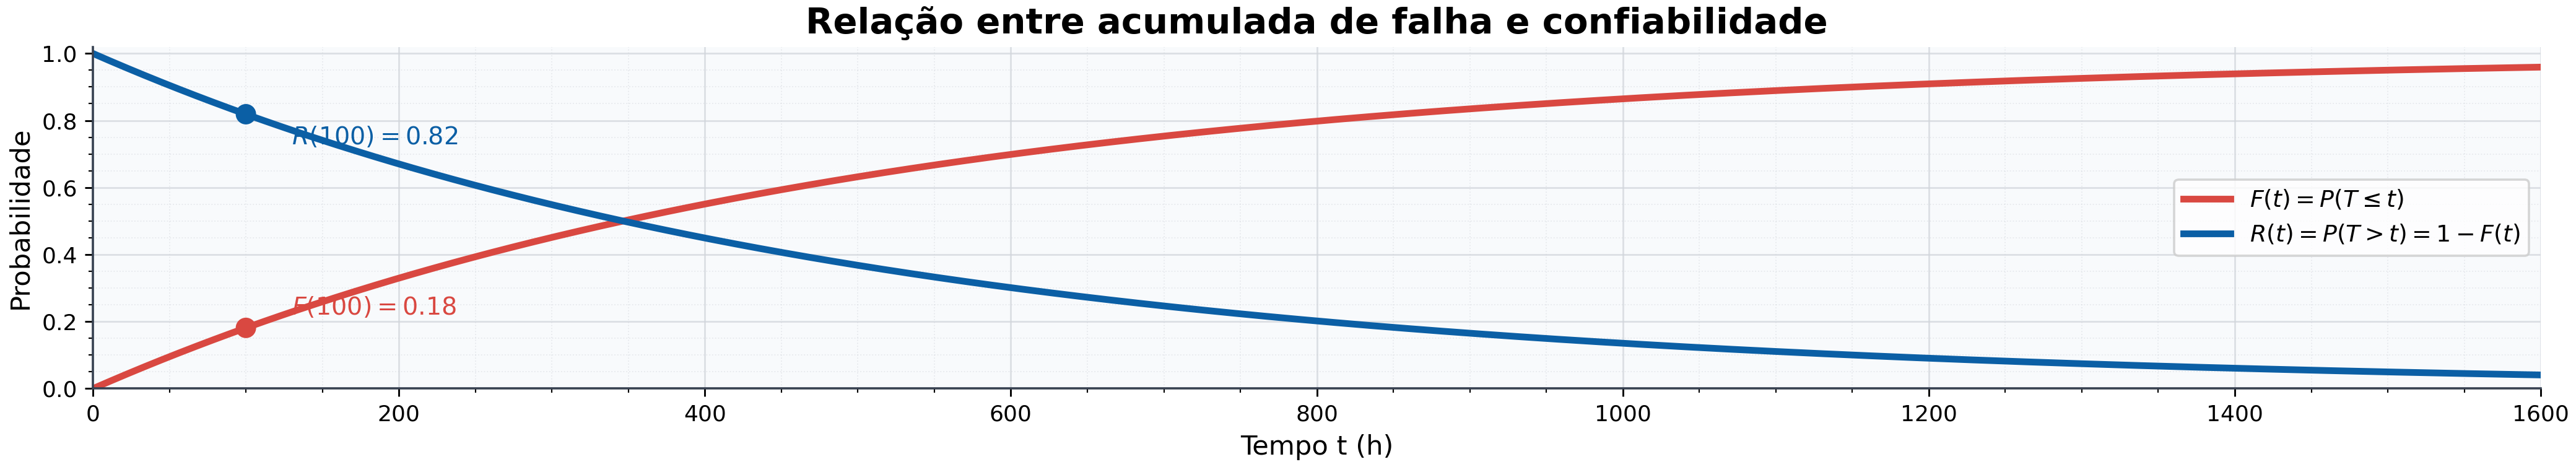
\includegraphics[width=\linewidth,height=0.35\textheight,keepaspectratio]{../img/unit2_cdf_reliability_wide.png}
\end{frame}

\begin{frame}{Passo 4: por que aparece a densidade \texorpdfstring{$f(t)$}{f(t)}?}
\begin{columns}[T,onlytextwidth]
\column{0.48\textwidth}
\[
f(t)=\frac{dF(t)}{dt}
\]
\begin{itemize}
  \item Como \(T\) é contínuo, usamos densidade.
  \item \(f(t)\) mostra \textbf{onde} a chance de falha se concentra.
  \item Não é probabilidade em um ponto isolado.
\end{itemize}
\begin{block}{Sem trauma matemático}
\(F(t)\) acumula, \(R(t)\) complementa e \(f(t)\) descreve a distribuição ao longo do tempo.
\end{block}
\column{0.52\textwidth}
\centering
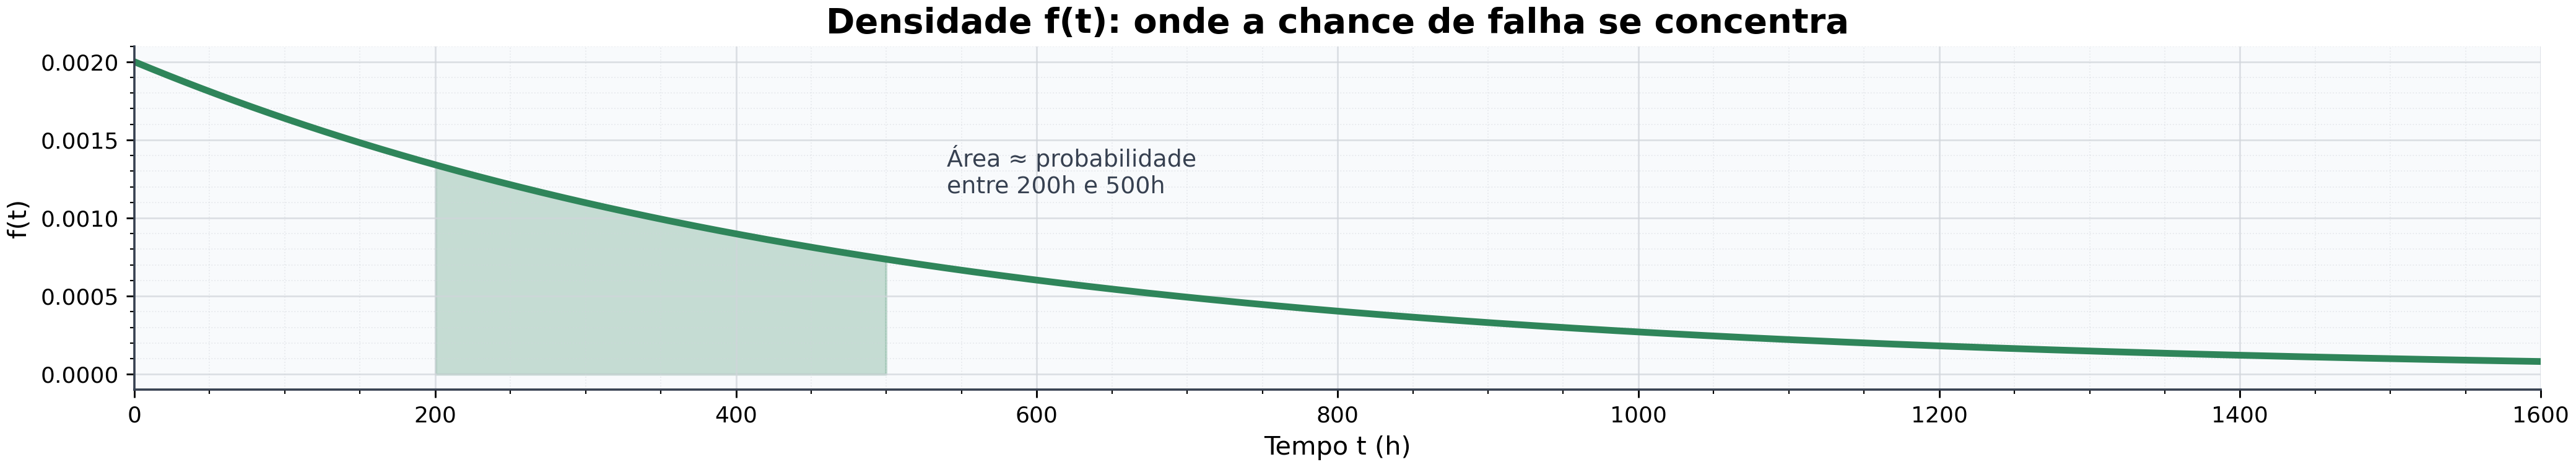
\includegraphics[width=\linewidth,height=0.35\textheight,keepaspectratio]{../img/unit2_density_wide.png}
\end{columns}
\end{frame}

\begin{frame}{Fault, Error, Failure e métricas médias}
\begin{itemize}
  \item \textbf{Fault $\rightarrow$ Error $\rightarrow$ Failure}
  \begin{itemize}
    \item Fault: causa latente.
    \item Error: estado interno incorreto.
    \item Failure: desvio percebido no serviço.
  \end{itemize}
  \item \(\MTTF\): tempo médio até falha (item não reparável).
  \item \(\MTBF\): tempo médio entre falhas (sistema reparável).
\end{itemize}
\end{frame}

\begin{frame}{Modelo exponencial: o mínimo necessário}
\begin{block}{Assunção comum em exercícios}
Taxa de falha aproximadamente constante.
\end{block}
\[
\lambda=\frac{1}{\MTBF}
\]
\[
\R(t)=e^{-\lambda t}=e^{-t/\MTBF}
\]
\begin{itemize}
  \item \(\lambda\): taxa de falha por hora.
  \item \(\MTBF\) maior \(\Rightarrow\) curva cai mais devagar.
\end{itemize}
\centering
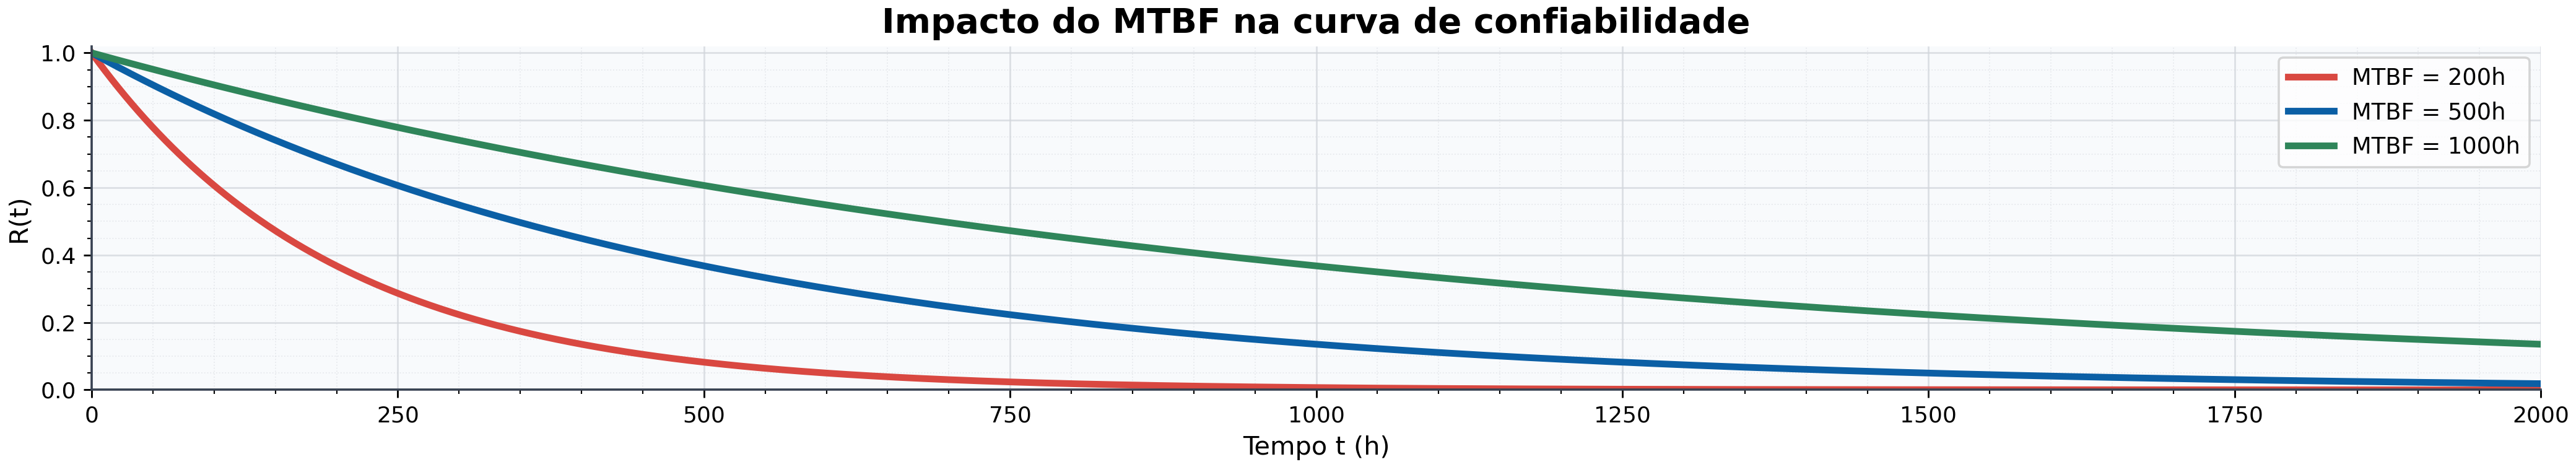
\includegraphics[width=\linewidth,height=0.35\textheight,keepaspectratio]{../img/unit2_mtbf_comparison_wide.png}
\end{frame}

\begin{frame}{Exemplo guiado de \texorpdfstring{$R(t)$}{R(t)} (passo a passo)}
Dados: \(\MTBF=500\,h\). Logo:
\[
\R(t)=e^{-t/500}
\]
\begin{enumerate}
  \item Para \(t=100\,h\): \(R(100)=e^{-0.2}\approx 0.8187\) (81,87\%).
  \item Para \(t=500\,h\): \(R(500)=e^{-1}\approx 0.3679\) (36,79\%).
\end{enumerate}
\begin{center}
  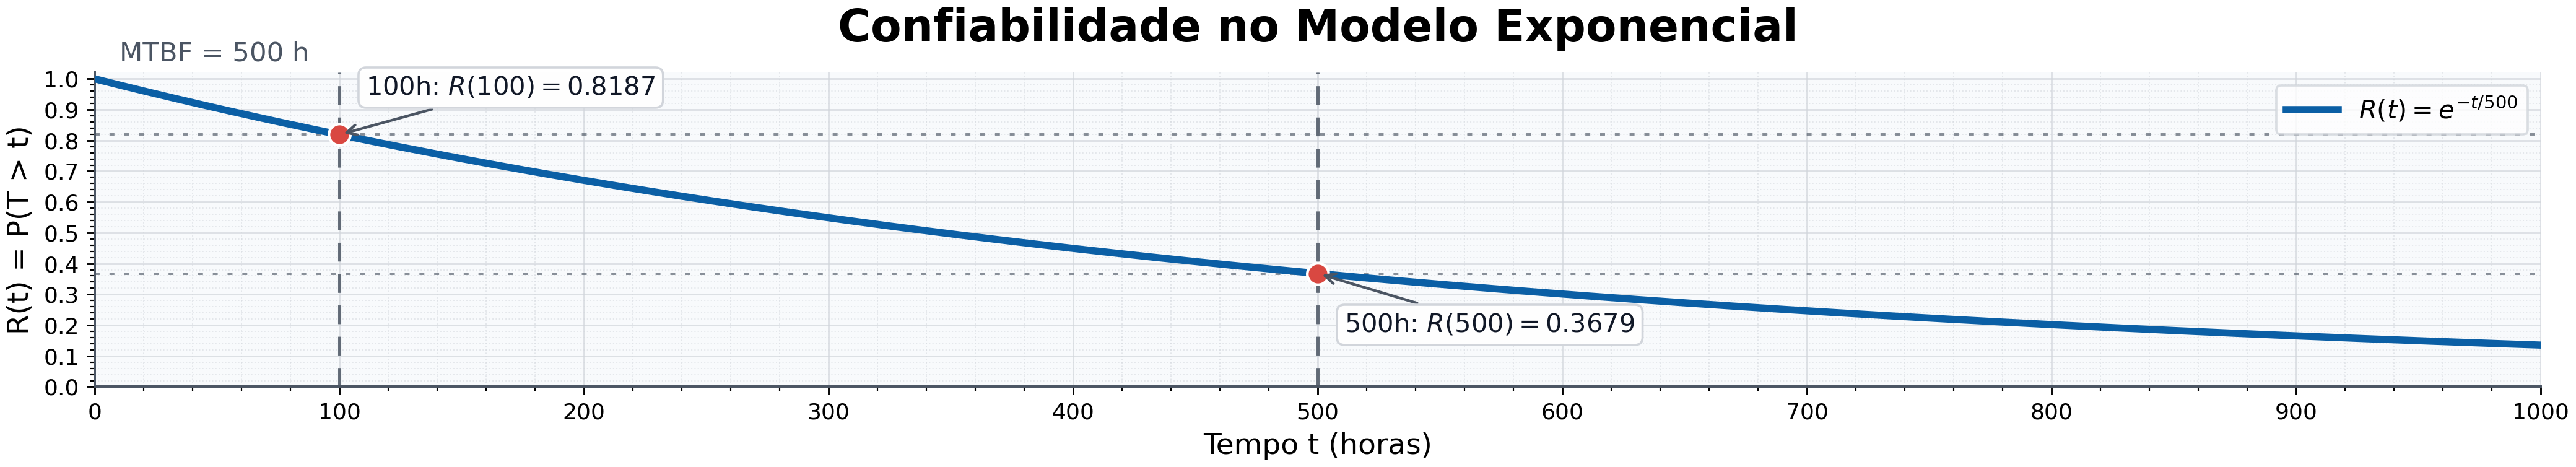
\includegraphics[width=\linewidth,height=0.35\textheight,keepaspectratio]{../img/reliability_curve_mtbf500_wide.png}
\end{center}
\end{frame}

\section{Disponibilidade}

\begin{frame}{Conceito e fórmula prática de disponibilidade}
\begin{block}{Disponibilidade (Availability)}
Fração de tempo em que o sistema está operacional.
\end{block}

\begin{itemize}
  \item \(\MTTR\): tempo médio para reparar/restaurar o serviço.
  \item Aproximação muito usada:
\[
\A \approx \frac{\MTBF}{\MTBF+\MTTR}
\]
\end{itemize}

\begin{block}{Contraste explícito}
Confiabilidade foca em \textit{não falhar}.\\
Disponibilidade foca em \textit{estar no ar}, mesmo após falhas, desde que o reparo seja rápido.
\end{block}
\end{frame}

\begin{frame}{SLA e indisponibilidade anual}
\begin{itemize}
  \item Se \(\A\) é conhecido, o downtime anual aproximado é:
\[
\text{downtime/ano} \approx (1-\A)\times 365\times 24\,h
\]
  \item Essa conta ajuda a traduzir percentual em impacto real de negócio.
\end{itemize}

\small
\centering
\begin{tabular}{l c}
\toprule
\(\A\) & Downtime aproximado por ano \\
\midrule
99\% & 87.6 h \\
99.9\% & 8.76 h \\
99.99\% & 0.876 h (52.6 min) \\
\bottomrule
\end{tabular}
\end{frame}

\section{Verificação de compreensão}

\begin{frame}{Verificação rápida de compreensão}
\begin{enumerate}
  \item Sistema A falha 10x mais, mas recupera 100x mais rápido.\\
  \textbf{Quem tende a ter maior disponibilidade?}
  \item Alta confiabilidade garante alta disponibilidade?\\
  \textbf{Não necessariamente}: \(\MTTR\) alto pode derrubar \(\A\).
\end{enumerate}

\begin{block}{Objetivo desse bloco}
Checar interpretação de engenharia, não apenas substituição em fórmula.
\end{block}
\end{frame}

\section{Exercícios e resolução guiada}

\begin{frame}{Exercício 1: MTBF, MTTR e \texorpdfstring{$\A$}{A}}
Um sistema operou por 30 dias. Houve 6 falhas.\\
Tempos de reparo (h): 1.0, 0.5, 2.0, 1.5, 1.0, 0.5.

\begin{enumerate}
  \item Estime \(\MTBF\) em horas.
  \item Estime \(\MTTR\) em horas.
  \item Calcule \(\A\).
\end{enumerate}
\end{frame}

\begin{frame}{Gabarito Exercício 1}
\begin{itemize}
  \item Total de horas: \(30\times24=720\,h\)
  \item \(\MTBF\approx 720/6=120\,h\)
  \item \(\MTTR=(1+0.5+2+1.5+1+0.5)/6=6.5/6=1.083\,h\)
  \item \(\A\approx \frac{120}{120+1.083}=0.9911\approx 99.11\%\)
\end{itemize}
\end{frame}

\begin{frame}{Exercício 2: Disponibilidade e SLA}
Uma plataforma tem \(\MTBF=200\,h\) e \(\MTTR=4\,h\).

\begin{enumerate}
  \item Calcule \(\A\).
  \item Estime o downtime por ano.
\end{enumerate}
\end{frame}

\begin{frame}{Gabarito Exercício 2}
\begin{itemize}
  \item \(\A=\frac{200}{200+4}=\frac{200}{204}\approx 0.98039\) (98.04\%)
  \item \(\text{downtime/ano}\approx (1-0.98039)\times8760\approx171.8\,h/ano\)
  \item Aproximadamente \textbf{7.2 dias/ano} indisponível.
\end{itemize}
\end{frame}

\begin{frame}{Exercício 3: \texorpdfstring{$\R(t)$}{R(t)} no modelo exponencial}
Assuma falhas exponenciais e \(\MTBF=500\,h\).
\begin{enumerate}
  \item Qual a probabilidade de operar sem falhar por 100 h?
  \item E por 500 h?
\end{enumerate}
\end{frame}

\begin{frame}{Gabarito Exercício 3}
\[
\R(t)=e^{-t/\MTBF}
\]
\begin{itemize}
  \item \(\R(100)=e^{-0.2}\approx 0.8187\)
  \item \(\R(500)=e^{-1}\approx 0.3679\)
\end{itemize}
\end{frame}

\begin{frame}{Exercício 4: melhorar \texorpdfstring{$\MTBF$}{MTBF} ou \texorpdfstring{$\MTTR$}{MTTR}?}
Comparar duas opções a partir do baseline \(\MTBF=100\,h\), \(\MTTR=5\,h\):
\begin{itemize}
  \item Opção A: aumentar \(\MTBF\) de 100 para 200 h (\(\MTTR=5\,h\)).
  \item Opção B: reduzir \(\MTTR\) de 5 para 1 h (\(\MTBF=100\,h\)).
\end{itemize}
Pergunta: qual melhora mais a disponibilidade?
\end{frame}

\begin{frame}{Gabarito Exercício 4}
\begin{itemize}
  \item \(\A_{old}=\frac{100}{100+5}=0.95238\)
  \item \(\A_A=\frac{200}{200+5}=0.97561\) (ganho de +2.323 p.p.)
  \item \(\A_B=\frac{100}{100+1}=0.99010\) (ganho de +3.772 p.p.)
\end{itemize}
\begin{block}{Conclusão}
Neste cenário, \textbf{reduzir MTTR} melhora mais a disponibilidade.
\end{block}
\end{frame}

\section{Fechamento}

\begin{frame}{Fechamento: pontos-chave}
\begin{enumerate}
  \item \(\MTBF\uparrow\) melhora confiabilidade e ajuda disponibilidade.
  \item \(\MTTR\downarrow\) melhora disponibilidade e pode ser mais custo-efetivo.
  \item \(\R(t)\) responde: \textit{qual a chance de não falhar até t?}
  \item \(\A\) e downtime traduzem engenharia para impacto operacional e SLA.
\end{enumerate}
\end{frame}

\begin{frame}{Gancho para a próxima aula}
\begin{itemize}
  \item Hoje: confiabilidade e disponibilidade com falhas acidentais e reparo.
  \item Próxima aula: \textbf{safety}, \textbf{security} e \textbf{resiliência}.
  \item Mensagem-chave: nem toda falha é acidental; ameaças e danos mudam o modelo.
\end{itemize}
\end{frame}

\begin{frame}{Referências base}
\small
\begin{itemize}
  \item Avizienis et al. (2004), \textit{Basic Concepts and Taxonomy of Dependable and Secure Computing}.
  \item NIST Handbook (conceitos de confiabilidade/disponibilidade).
  \item Materiais de SRE sobre disponibilidade e impacto de indisponibilidade.
\end{itemize}
\end{frame}

\end{document}
